% LaTeX template for thesis and dissertation ETDs
% Created by Benjamin Hilburn ( bhilburn@vt.edu )

\documentclass[pdftex,12pt,onecolumn]{report}

\setlength{\textwidth}{6.5in}
\setlength{\textheight}{8.5in}
\setlength{\evensidemargin}{0in}
\setlength{\oddsidemargin}{0in}
\setlength{\topmargin}{0in}
\setlength{\parindent}{0pt}
\setlength{\parskip}{0.1in}
\usepackage{setspace}
\renewcommand{\baselinestretch}{2}

\usepackage{cite}
\usepackage{makecell}
\usepackage{multicol}
\usepackage{textcomp}

\usepackage{palatino}
\fontsize{12}{14}

\usepackage[pdftex]{graphicx}
\usepackage[center]{caption}
\usepackage{float}
\graphicspath{{./images/}}
\DeclareGraphicsExtensions{.pdf,.jpeg,.png}

\usepackage{longtable}

\renewcommand{\arraystretch}{1.5}

\usepackage[cmex10]{amsmath}
\usepackage{algorithmic}
\usepackage{algorithm}

\usepackage{listings}
\usepackage{csvsimple}

\usepackage{array}
\usepackage{mdwmath}
\usepackage{mdwtab}


\usepackage[font=footnotesize]{subfig}
\usepackage{url}


\usepackage[breaklinks]{hyperref}
\hypersetup{
    unicode=true,         							% non-Latin characters
    pdftoolbar=true,								% show Acrobat�s toolbar?
    pdfmenubar=false,								% show Acrobat�s menu?
    pdffitwindow=false,								% window fit to page on open
    pdftitle={Creating Socio-Technical Patches for Information Foraging: A Requirements Traceability Case Study},			% title
    pdfauthor={Darius Cepulis},						% author
    pdfsubject={M.S. Thesis of Computer Science},	% subject
    pdfcreator={Darius Cepulis},					% creator of the document
    pdfnewwindow=true,								% links in new window
    colorlinks=true,								% false: boxed links; true: colored links
}
\urlstyle{same}

\begin{document}

\thispagestyle{empty}
\pagenumbering{roman}
\begin{center}
{\Large 
Creating Socio-Technical Patches for Information Foraging: \\ A Requirements Traceability Case Study
}
\vfill
Darius Cepulis \\
B.S. Computer Engineering, University of Cincinnati, 2018
\vfill
Dr. Nan Niu, Chair \\
Dr. Carla Purdy \\
Dr. Chia Han  
\vfill
Thesis submitted to the Faculty of the \\
University of Cincinnati  College of Engineering and Applied Science \\
in partial fulfillment of the requirements for the degree of
\vfill
Master of Science \\
in \\
Computer Science
\vfill
July 13th, 2018 \\
Cincinnati, OH
\end{center}
\pagebreak


\thispagestyle{empty}
\begin{singlespace}
\begin{center}
{\large Creating Socio-Technical Patches for Information Foraging: \\ A Requirements Traceability Case Study}
\\
Darius Cepulis
\vfill
ABSTRACT
\end{center}
Work in information foraging theory presumes that software developers have a predefined patch of information (e.g., a Java class) within which they conduct a search task. However, not all tasks have easily delineated patches. Requirements traceability, where a developer must traverse a combination of technical artifacts and social structures, is one such task. We examine requirements socio-technical graphs to describe the key relationships that a patch should encode to assist in a requirements traceability task. We then present an algorithm, based on spreading activation, which extracts a relevant set of these relationships as a patch. We test this algorithm in requirements repositories of four open-source software projects. Our results show that applying this algorithm creates useful patches with reduced superfluous information. 
\\
Keywords: Information foraging theory, Spreading activation, Requirements Traceability
\vfill
\pagebreak
\begin{center}
\vfill
Copyright 2018, Darius Cepulis
\end{center}
\pagebreak
\end{singlespace}


\chapter*{Acknowledgments}
A big thanks to Kristin, who turned my doodles into figures while I was furiously writing.\\\\
A huge thanks to Dr. Niu's research team, who put together an enormous and useful database and answer set. All I had to do was query.\\\\
Finally, an enormous thanks to Dr. Niu, who provided the ideas that formed the backbone of this paper, and the guidance that made sure it got done.

\chapter*{Dedication}

To Kristin, Stefan, Mom, Dad, Alex, Ryan, Stack Overflow, Audrey, Sofia, and iOS 12.

\tableofcontents
\pagebreak
\pagebreak

\listoffigures
\pagebreak

\listoftables
\pagebreak

\pagenumbering{arabic}
\pagestyle{myheadings}

\chapter{Introduction}
\markright{1. Introduction \hfill }
% - Welcome to Information Foraging
If we understand how a user seeks information, then we can optimize an information environment to make that information easier to retrieve. Pirolli and Card worked to understand information-seeking by defining information foraging theory~\cite{ift}.
Information foraging theory describes a user's information search by equating it to nature's optimal foraging theory: in the same way that scent carries a predator to a patch where it may find its prey, a user follows cues in their environment to information patches where they might find their information.

% - Patches Patches Patches Patches
Information foraging theory has seen many applications since Pirolli's seminal work. For example, in web search, foragers follow information scent to their patches, web pages~\cite{pirolliWeb,wufis}. Understanding how foragers find information in web search has helped developers design the information environment of their web pages~\cite{wufis}. In code navigation and debugging, information foraging theory describes how developers seek to resolve a bug report by navigating from fragment to fragment of code to define and fix the problem~\cite{navValueCost}.
By understanding the process of finding and fixing bugs, models can be written to assist in this process~\cite{pfisRevisit}. In both of these scenarios, the patch is clearly defined: in web search, a forager's patch is a web page, and in debugging, a developer's patch might be a fragment of code. What happens, though, when the patch is not clearly defined?

% - We don't have patches in socio-technical systems
Consider socio-technical systems, where information artifacts are connected to people. Facebook, YouTube, Twitter, GitHub, and Wikipedia all have information artifacts, like posts and code snippets, with a rich context of social interactions tying them together. A forager traverses both the artifacts and the social structures behind them in an information seeking task. Therefore, both artifacts and social structures should be considered when defining a patch, and patches are not necessarily immediately evident. Consider a user wondering how a reposted image became so popular among their friends: how could patches be defined for this forager? Photos, posts, comments, friends' connections? A GitHub code fragment or Facebook Friend can't answer these questions alone, so patches must consist of some combination. In this paper, we describe a method for delineating such patches.

% - RT is a socio-technical system! RT is important
Requirements traceability is an ideal field for examining patch creation in a socio-technical environment. Requirements traceability is a socio-technical system used to describe and follow the life of a requirement by examining the trail of artifacts and people behind them, from the requirement's inception to implementation. Requirements traceability problems, as studied by Gotel and Finkelstein~\cite{ICSE30}, arise when questions about the production and refinement of requirements cannot be answered. More specifically, with a traceability failure, US Food and Drug Administration might cast doubt in product safety~\cite{ICSE46}. With a traceability failure, the CEO of a prominent social media company cannot explain to Congress how a decision to withhold information from customers was made~\cite{politicoFacebook}. Applying information foraging to these problems could significantly increase efficiency and efficacy of these traceability tasks.

% - Start defining RT in terms of foraging. patch patch patch patch.
We relate requirements traceability to information foraging theory and its patches by considering requirements traceability questions. We define a requirements traceability question as a query that a project stakeholder issues \textit{in situ} wanting to know a requirement's life. A requirements traceability question is where a user's traceability task becomes a foraging task; the question represents the user's information need, or foraging prey. If questions represent a traceability forager's prey, what represents a traceability forager's patch? Put simply, we aim to answer the research question: \textit{where should a user search to understand their requirements traceability question?}

% - Our contribution
This paper makes two contributions by deriving a method for delineating these patches. First, by examining requirements socio-technical graphs constructed from four requirements repositories containing 125 traceability questions, we identify classes of relationships that should be considered in similar requirements traceability tasks. Second, we derive an algorithm, based on spreading activation, which combines these classes with information foraging concepts to create relevant patches where foragers can conduct their traceability tasks. The patches that our algorithm produces are as small as 5-10 nodes\textemdash a manageable quantity for a forager\textemdash representing knowledgeable users and useful information artifacts. The method for identifying these classes and deriving this algorithm can be extended to other socio-technical tasks.

\chapter{Background}
\markright{2. Background \hfill}
\section{Information Foraging}
Information Foraging Theory (IFT)~\cite{pirolli07} simplifies, in a principled way, analyzing information-seeking tasks by providing constructs borrowed from its optimal foraging theory roots. Optimal foraging theory describes predators that pursue prey through an environment, following scent from locality to locality. The predator is always trying to optimize their task. In IFT, the information seeker pursues information through an information environment. Scent, in the information environment, is a construct that exists in the forager's mind, representing their perception of where they might find information; this perception is shaped by proximal cues\textemdash hints provided by the information environment. Information foragers follow scent from locality to locality, information patch to information patch, pursuing their prey. 

Consider the following analogy: a forager is seeking berries. They go to a patch of berries, and estimate how many berries might be in that patch. They then pick berries until they decide that they have picked enough from this patch, and should move to the next one. In this model, proximal cues (how full the patch looks, how many berries nearby patches had), or scent, indicate to the forager how many berries might be in that patch. Of course, the forager might not estimate correctly how many berries there are if the indications are misleading, and they might switch to another patch too early (still easy berries to pick) or too late (time wasted looking for berries instead of switching patches). Building a correct estimate, and making berries easy to pick, so to speak, is an important application of IFT. 

The constructs provided by IFT were first used to analyze how a web user might search for information online~\cite{pirolliWeb}, modeling scent as relatedness of a link to the forager's prey. This work eventually developed into the WUFIS (Web User Flow by Information Scent) algorithm~\cite{wufis}. WUFIS represents network topology as a graph, where nodes are web pages and edges are the links that a user can click to navigate from one to another. IFT's scent is represented by relatedness of the words in a webpage to the forager's information need. The algorithm then predicts where the user will navigate by applying spreading activation. 

\begin{figure}
	\centering
	\includegraphics[width=0.5\linewidth]{spreading_example.png}
	\caption{Example of Spreading Activation in Neuroscience. ``Dog'' is initially activated; darker shading indicates higher activation. Source: ~\cite{spreadingexample}}
	\label{fig:activation}
\end{figure}

Spreading activation is a concept borrowed from neuroscience: Collins and Loftus ~\cite{spreadingactivation} posited that all memories and knowledge in our minds are connected in a network, and activating one memory also activates neighboring memories. Spreading activation, as adapted by the Information Foraging world, works by assigning one (or several) nodes in a graph with an initial activation of 1. Each edge in the graph is assigned with a weight. In the case of WUFIS, the weight is proportional to the similarity of the two nodes that the edge is connecting. In other cases, all edges are assigned the same weight. Each node in the graph is traversed, and the activation is ``spread'' to its children: typically, the parent node's activation is multiplied by the weight so that the child node's activation is lower. Each node, then, has an activaiton value that represents its similarity to the originally-activated node, as dictated by proximity to the original node and edge-weights. This mechanism can be seen in Figure \ref{fig:activation}. For WUFIS, spreading activation assigns each node with a value which represents the probability that a forager, given their current location and information need together with the scent of links connecting pages, will navigate to a specific page.

This spreading activation concept was utilized to model programmer navigation in the development of PFIS~\cite{pfis1a} and its subsequent revisions~\cite{pfis2,pfis3a}. PFIS built upon the spreading activation of WUFIS by applying it to the field of developer navigation~\cite{pfis1a}, inferring the forager's goal~\cite{pfis2}, and creating multi-factor models with PFIS~\cite{pfis3a}. In the programmer navigation domain, WUFIS web page nodes were now code fragments, and its edges were any click-able link that would navigate a developer from one fragment to another. When inferring the forager's goal, PFIS authors introduced the concept of heterogeneity to their network: in addition to linking code fragments, the PFIS algorithm also linked code fragments to key words (e.g., those extracted from a bug report), creating a more nuanced topology. Inspired by this heterogeneous approach, we take spreading activation to the socio-technical realm.

\section{Socio-Technical Networks}
In order to develop a spreading activation algorithm to answer requirements traceability questions in the socio-technical realm, we first examine work conducted in socio-technical graphs. Both Herbsleb and colleagues' socio-technical theory of coordination (STTC) ~\cite{herbsleb16}, and the Codebook project ~\cite{codebook} attempt to answer requirements traceability questions with socio-technical models. We begin by examining Herbsleb et al.'s work.

Herbsleb et al. conduct their work examining dependencies among engineering decisions\textemdash ``Who should work with whom?''. They answer this question by defining a constraint satisfaction problem that people must organize to solve. The theory draws from the key observation that the number of people was a powerful predictor of coordination problems (e.g., delay in development ~\cite{herbsleb03}), and quantifies people’s working relationships via a dependency network of work items. The solution to this problem provides an answer to the earlier ``Who should work with whom?'' question, which in turn serves as a unifying basis for solving a class of coordination problems, including expertise finding ~\cite{herbsleb02,herbsleb09}, cross-site communication ~\cite{herbsleb01}, and pull request acceptance in social coding environments ~\cite{herbsleb14}. While this STTC can address some of the traceability questions (e.g., ramifications ~\cite{ICSE30}), other questions that we want to answer, such as ``Which programmers are more error prone in their code according to the test results?'' ~\cite{lohar16}, need the relationships between people and artifacts. For a foundation that can answer all of our traceability questions, we turn to Codebook.

In the Codebook~\cite{codebook} project, people and work artifacts were ``friends'' in a social network. A user might be connected to an email they sent, bug they closed, and a commit they pushed; that commit has changes in code containing classes and calls. A sample Codebook topology can be seen in Figure \ref{fig:codebook}. By using a single data structure to represent these people, artifacts, and relationships, and a single algorithm (regular language reachability) to analyze this graph, Codebook could handle all the inter-team coordination problems identified in a survey responded by 110 Microsoft employees~\cite{codebook10}, including requirements traceability problems. 

\begin{figure}[ht!]
	\centering
	\includegraphics[width=0.5\linewidth]{codebook.png}
	\caption{The Codebook Topology, Source: ~\cite{codebook}}
	\label{fig:codebook}
\end{figure}

Codebook addresses problems by having a project personnel cast their coordination needs into regular expressions. For example, the requirements traceability question ``Which program manager wrote the specification for that code?'' could be addressed in Codebook with the regular expression ``\textsc{Code MentionedBy WordDocument AuthoredBy Person}''. This is a manual task, requiring a domain expert. In contrast, spreading activation can provide a mechanism for automated querying. We therefore adopt Codebook's underlying data structure, but instead of regular language reachability, we adapt the people-artifact graph for spreading activation.

\chapter{Examining Requirements Socio-Technical Graphs}
\markright{3. Examining RSTGs \hfill}
In order to successfully create patches in a requirements traceability environment, we must first understand the characteristics of the environment. To do this, we construct graphs of the environment following the Codebook paradigm. We then examine the types of human-human and human-artifact relationships that connect a traceability question to an identified answer; encoding these relationships can build a patch that a requirements traceability forager can explore to understand their prey\textemdash their need to understand their traceability question\textemdash better.

\section{The Information Environment}
\begin{table}[!b]
  \caption{Jira Projects and Characteristics}
  \centering
  \begin{tabular}{ |c|| c | c | c | c |  }
    \hline
    Project & Domain & Written & \makecell{Initial \& Latest\\Releases Examined} & \makecell{Questions} \\
    \hline
    \makecell{DASHBUILDER} & \makecell{data\\reports} & \makecell{Java,\\HTML} & \makecell{Aug 27, 2014 \& \\Apr 14, 2016} & 31 \\
    \hline
    DROOLS & \makecell{business\\rules} & Java & \makecell{Nov 13, 2012 \&\\Jul 17, 2017} & 57 \\
    \hline
    \makecell{IMMUTANT} & \makecell{complexity\\reduction} & Clojure & \makecell{Mar 14, 2012 \&\\Jun 23, 2017} & 18 \\
    \hline
    JBTM & \makecell{business\\process} & \makecell{Java,\\C++} & \makecell{Dec 5, 2005 \&\\Jul 14, 2017} & 5 \\
    \hline
  \end{tabular}
  \label{tab:jiraProjects}
\end{table}

\begin{table}[!t]
  \centering
  \small
  \caption{Select Questions with Identified Answers from DROOLS}
  \tabcolsep=0.11cm
  \scalebox{0.70}{
    \begin{tabular}{ |l|l|l|l|l|l|l|  }
      \hline
      id & issue & body & asker & answered by & role & operations \\
      \hline
      1206 & 972 & Can you please send a PR adding a new example...? \ldots & Mario Fusco & Mauricio Salatino & Creator & add pull request \\
      1220 & 963 & This should be fixed for 6.4.0.Final, does it sound possible? & Mauricio Salatino & Petr Siroky & Assignee & change fix version \\
      1371 & 907 & ...Please look at [my page]. What do you think\ldots & Michael Kiefer & Geoffrey De Smet & Creator & marked as done \\
      1377 & 905 & Thanks...[\textasciitilde martenscs]. Is there any other prefix?  \ldots & Petr Siroky & & & \\
      1383 & 901 & any news here [\textasciitilde mfusco]? & David naranjo & Geoffrey De Smet &  & provide opinion \\
      1627 & 823 & Hi Geoff, I don't know what shoud be the expected behaviour? \ldots & Michael Kiefer &  &  & \\  
      \hline
  \end{tabular}
  }
  \label{tab:drools}
\end{table}


% - Why Jira?
The literature suggests that issue trackers are essential for open-source projects to manage requirements~\cite{ICSE5,ICSE25,ICSE33,ICSE40,ICSE60}. Although the requirements of an open-source project can originate from emails, how-to guides, and other socially lightweight sources~\cite{ICSE62}, the to-be-implemented requirements ``eventually end up as feature requests in an issue-tracking system''~\cite{ICSE33}. We therefore turn to the issue-tracking system Jira, with issues like Figure \ref{fig:drools} to understand the life of requirements.

\begin{figure}
  \centering
  \includegraphics[width=\linewidth]{drools.png}
  \caption{A Screenshot of a Common Issue in Jira, in the DROOLS project. From this, we will take Issue, Assignee, Reporter/Creator, and questions like the first comment.}
  \label{fig:drools}
\end{figure}


% - Why 6 projects within Jira?
From Jira, we select four open-source projects from the Apache software foundation~\cite{ICSE7} or the JBoss family~\cite{ICSE38}.
The four projects tackle problems in different domains with implementations written in different programming languages, as seen in Table \ref{tab:jiraProjects}.

% - within projects, requirements manifest themselves as questions
Within the chosen projects, we focus on questions and answers. As discussed, questions represent a traceability forager's information need. By finding the exact person who answered a forager's question, we can gain insight into the information environment; we \textit{know} that the person who answered a traceability question can provide information on the traceability issue. For each project, two researchers identified comments that were questions (using tools from Stanford's CoreNLP project ~\cite{corenlp} to identify questions in multiple forms, e.g., with/without a question mark) and identified the respective answer comments, building their answer sets individually. Some examples of the answer sets generated can be seen in Table \ref{tab:drools}. The researchers reached a substantial degree of agreement (average Cohen's kappa=0.67) on requirements traceability questions over the 4 projects. Discrepancies were resolved in a joint meeting between the researchers. 

With our information environment identified, the next step to creating patches is to build a requirements socio-technical graph (RSTG) so that we can inspect the topology of the environment using graph theory concepts. A graph requires nodes and edges.

\section{Constructing Requirements Socio-Technical Graphs}
\subsection{Nodes}
% - why do we considered these projects heterogeneously? 
% - what are our node types? issues, comments, and people.
In Jira, issues (typically tasks or feature requests) are our requirements. Comments are provided to the issue, and may contain questions or answers. Users create issues, are assigned to issues, submit comments, and reference other users within their comments. This process can be seen in the screenshot of a typical Jira issue in Figure \ref{fig:drools}. Contemporary approaches to requirements traceability are either artifact-based (e.g., trace retrieval) and would consider only the comments and issues~\cite{ICSE15}, or are driven by social roles (e.g., contribution structures in the requirements specification production) and would consider the relationships of the people~\cite{ICSE29}. As we constructed our answer set, however, we realized the impact of the people-artifact relationships on the ability to track a requirement's life. Therefore, we consider Jira's issues, comments, \textit{and} people in our information environment. These will serve as our nodes. What, then, serve as our edges?

\subsection{Edges}

\begin{figure}
	\centering
	\includegraphics[width=\linewidth]{rstg.pdf}
	\caption{Requirements Socio-Technical Graph}
	\label{fig:rstg}
\end{figure}

By manually inspecting the paths between questions and their eventual answers, we are able to define the edges in our network topology. Consider the following example: Figure \ref{fig:rstg} is a subgraph from the IMMUNANT project, showing two questions and their answers. User 2881 created Issue 73650. User 6655, the forager, commented on the issue (Comment 149789), asking User 2881 for clarification by referencing them in the comment. User 2881 commented on the issue (Comment 149790), providing the clarification. In another foraging interaction, User 2881, now the forager, commented on the issue (Comment 149792), asking ``This is now available in [incremental build | http://immutant.org/builds/2x/] 591 and newer. Can you give that a try and confirm it works for you?'' User 6655 responded (Comment 149793) ``I've finally found the time to test this and can confirm it works! Thanks!''. 

These two foraging interactions demonstrate most of the relationships that we observed between nodes in the datasets. These relationships are treated as the edges within our graph:
\begin{samepage}
\begin{itemize}
  \item \textit{Creator:} Users create issues
  \item \textit{Commented, Asked: }Users post comments and questions
  \item \textit{Comment, Question:} Comments and questions are posted to Issues
  \item \textit{Referenced:} Comments can reference other users
  \item \textit{Assignee:} (Not pictured) Users can also be designated assignees on issues 
\end{itemize}
\end{samepage}
While some relationships could be considered as unidirectional, e.g., a user posting a comment, the comment also serves as a bridge connecting the issue to the user, who is knowledgeable on the issue. We therefore elected to encode the network as an undirected graph.

\subsection{Scripting Graph Construction}
With our desired node and edge types identified, we then automated graph construction in Python, leveraging the graph construction and analysis library, NetworkX ~\cite{networkx}, heavily. The full code described here can be found in our online repository ~\cite{repo}, as well as in Appendix \ref{app:python}. Our objective was to automate the construction of RSTGs like Figure \ref{fig:rstg} for each question, representing the state of the project at the time of the question. Representing the network at the time of the question was important to us so that only relationships that had existed prior to asking of the question would be considered.

In order to construct RSTGs, our script queried a database that held tables with the following characteristics. Note that irrelevant tables have been omitted:
\begin{itemize}
  \item \textit{jira\textunderscore issue:} All projects' issues, as well as assignee, creator, and a description
  \item \textit{jira\textunderscore issue\textunderscore comment:} All comments, as well as who posted them on which issue
  \item \textit{jira\textunderscore issue\textunderscore type:} Issue types, e.g., ``Bug'', ``New Feature'', ``Improvement''
  \item \textit{jira\textunderscore project:} Keys of projects in database, as well as names and descriptions. 
  \item \textit{jira\textunderscore user:} All of users' usernames, real names, and database IDs
\end{itemize}

We began by pulling all of a project's issues and associated users and adding them to a graph (\texttt{dbManager.addProjectIssuesToGraph(project,graph)}). This was performed by querying the database (\textsc{select * from jira\textunderscore issue where project = x}) and adding a node for each result, each result's creator, and each result's assignee. The creators and assignees were connected to their issue with a labeled edge.

Next, each comment was added to the graph, and was connected to its issue, author, and any referenced user (\texttt{dbManager.addProjectCommentsToGraph(project,graph)}) with the query \textsc{select * from jira\textunderscore issue\textunderscore comment where issue in ( select id from jira\textunderscore issue where project = x )}. While each issue has its creator and assignee explicitly defined by Jira, and each comment has its author and issue, some additional processing was required to identify references. In practice, a reference can either be the user's username (e.g., [\textasciitilde ge0ffrey]) or first name (e.g., ``Geoffrey,'' or ``Geoffrey:''). With regular expressions (\texttt{\textbackslash {[}\textasciitilde (.+?)\textbackslash {]}}), usernames were identified in the body of a comment and connected the comment to the user. However, a dictionary of first-name references had to be manually built so that an identified reference (regex: \texttt{{[}A-Z{]}{[}a-z{]}+?,|{[}A-Z{]}{[}a-z{]}+?:}) could be connected to its user. 

\section{Properties of Requirements Socio-Technical Graphs in Information Foraging}
We now tie our RSTGs to information foraging theory. When a forager asks a question, like the ones in Figure \ref{fig:rstg}, where do they find their answer? The location of the answer might grant us insight on what we should include in a patch of information relevant to a question. What path might the traceability forager typically follow to the user who will provide the answer, gathering information on their prey along the way?

\begin{figure}
	\centering
	\includegraphics[width=\linewidth]{pie.png}
	\caption{Degrees of Separation between Question and Answer in Projects}
	\label{fig:pie}
\end{figure}

By analyzing the paths connecting question nodes and answer nodes, we identified recurring patterns connecting traceability questions with answers. The patterns are organized by degrees of socio-technical separation, which we define as the minimum number of edges to be traversed between two nodes. Figure \ref{fig:pie} displays the frequency of degrees separating questions and answers for our 125 questions. 

\subsection{One or Two Degrees of Separation From Question}
Figure \ref{fig:pie} shows that more than three-quarters of answers are within two degrees of the question. These represent simple foraging tasks. By the time a forager posts a question, they may be relatively familiar with an issue. The very fact that they chose a specific issue to comment on demonstrates that they expect their answer to be near the issue. A well-informed forager will often reference the exact user they expect to know the answer. These kinds of relationships fall within this category.

\begin{figure}[ht]
	\centering
	\includegraphics[width=\linewidth]{1deg.pdf}
	\caption{Referenced (1 Degree)}
	\label{fig:1deg}
\end{figure}

Within one degree of the question, two types of answers were observed. The first is when the forager answers their own query. Because the forager, in the RSTG, is directly connected to their comment, this is one degree of separation. The second is when a user is referenced within a comment. As shown in Figure \ref{fig:1deg}, when a user is referenced in a comment, they are directly connected to the comment. Comment 70842, from the DROOLS project, is a good example of this: "What should the URL look like in your opinion [\textasciitilde tirelli]?" asks User 4079. User tirelli answers. A vast majority of the 31\% of answers one degree away from the question came from direct references.

\begin{figure}[ht]
	\centering
	\includegraphics[width=\linewidth]{2deg.pdf}
	\caption{Creator or Assignee (2 Degrees)}
	\label{fig:2deg}
\end{figure}

Within two degrees of separation, we observed two more types of answers: when a forager asks a question on an issue, either the issue creator or issue assignee often responds. Figure \ref{fig:2deg} shows this interaction. When a forager posts a question to an issue without a reference, the creator, with their knowledge of what the issue is, or the assignee, with knowledge of what is being done to solve the issue, can answer. In Comment 353748, from the JBTM project, User 133 posts to an issue: ``Status update please?'' User 3619, assignee, provides an answer.

\subsection{Collaborators and Contributors\textemdash Three or Four Degrees of Separation From Question}
More challenging foraging occurs when the user with the answer is three or more degrees of separation away from the question. With each degree, the number of information artifacts and other users a forager must traverse increases exponentially. Identifying patterns and presenting useful patches to the forager in this class of foraging presents far greater potential. We present a few of the most frequent types of interactions that occur within this radius. 

\begin{figure}[ht]
	\centering
	\includegraphics[width=\linewidth]{3degCollab.pdf}
	\caption{Frequent Collaborator of Asker or Referenced User (3 Degrees)}
	\label{fig:3degCollab}
\end{figure}

Most answers in our projects within three degrees of separation were of the type shown in Figure \ref{fig:3degCollab}: Comment--Person--Issue--Person. The question connects to a person\textemdash either the traceability forager or a referenced user\textemdash and the answer comes from a \textit{Frequent Collaborator}. While neither the forager themselves nor a referenced user has an answer, someone they collaborate with does. The Collaborator is connected with the user or the referenced by one or more comments (where the Collaborator is directly referenced). We notice that Collaborators are often highly-central users in a project, whose Frequent Collaborator status arises from their frequent contributions to projects. In other words, they are Frequent Collaborators because they are frequent users in general.

\begin{figure}[ht]
	\centering
	\includegraphics[width=\linewidth]{3degContrib.pdf}
	\caption{Frequent Contributor to Issue (3 Degrees)}
	\label{fig:3degContrib}
\end{figure}

The second type of answer within three degrees of separation is that shown in Figure \ref{fig:3degContrib}: Comment--Issue--Comment--Person. We call this type of answer a \textit{Frequent Contributor}. This user does not directly know the forager, nor are they creator or assignee of the issue. However, the Contributor has commented and asked on a given issue one or more times. Again, Frequent Contributors tend to be highly-central users. Figure \ref{fig:pie} shows that Frequent Collaborators and Frequent Contributors represent 11\% of answers in our dataset.

\begin{figure}[ht]
	\centering
	\includegraphics[width=\linewidth]{4degCollab.pdf}
	\caption{Frequent Collaborator of Creator or Assignee (4 Degrees)}
	\label{fig:4degContrib}
\end{figure}

Within four degrees, we see another variant of The Collaborator: a \textit{Frequent Collaborator of the Creator or Assignee} (Figure \ref{fig:4degContrib}). This type of relationship is signified by the pattern Comment--Issue--Person--Issue--Person. The creator or assignee of the issue has collaborated with the answerer on other issues before, either as creator or assignee on those issues. While the creator or assignee of the primary issue being considered may not have the answer, someone they often work with may. Figure \ref{fig:pie} shows that these kinds of interactions represent 3\% of our dataset.

We hypothesize that, within three or four degrees of separation, several other types of collaborators could be observed. Frequent Collaborators of the Asker could manifest by Comment--Person--Comment--Person, rather than Comment--Person--Issue--Person as we observed. Within four degrees, we observed Frequent Collaborators of Creators or Assignees; a Frequent Collaborator of the Asker could also show up within four degrees (Comment--Person--Issue--Comment--Person, or Comment--Person--Comment--Issue--Person). 


\subsection{Five or More Degrees of Separation}
In our sample set of 125 questions, there were no instances of five or more degrees of separation. Within this class, though, we hypothesize that more interesting variations of Frequent Collaborators and Frequent Contributors would arise; if one user does not know the answer, someone they know will. However, not having observed this class, we do not anticipate that it will be a commonplace sight.

\subsection{Unconnected Users}
\label{unconnectedusers}
\begin{figure}[ht]
	\centering
	\includegraphics[width=\linewidth]{disconnected.pdf}
	\caption{Answer disconnected from network}
	\label{fig:disconnected}
\end{figure}

The final pattern observed was one instance of an answer unconnected from the graph of the project (Figure \ref{fig:disconnected}). At the time the question was asked, the user who will eventually answer the forager's traceability question was not yet connected to the project by the relationships we chose to express as edges. (For example, in Appendix \ref{app:cytoscape}, Figure \ref{fig:c9396}, some users are not in the network at the time of that comment). When that user finally did connect to the the network, they were four degrees of separation away (Comment--Person--Comment--Issue--Person), appearing as the assignee to an issue where the asker had commented. With a larger dataset, these not-yet-connected relationships would be interesting to assess. More edge and node types could enable a connection between that user and the question.

\begin{table}[!ht]
	\caption{Number of Nodes Within N Degrees of Question}
	\centering
		\begin{tabular}{ |c||c|c|c|c|c|  }
		\hline
		& Min & Q1 & Med & Q3 & Max \\
		\hline
		2 Degrees & 4 & 29   & 192  & 442  & 1908 \\
		3 Degrees & 5 & 271  & 510  & 1405 & 4192 \\
		4 Degrees & 5 & 625  & 2288 & 3636 & 7542 \\
		5 Degrees & 5 & 1949 & 3084 & 4597 & 7950 \\
		\hline
	\end{tabular}
	\label{tab:radiusStats}
\end{table}

It appears, from these classes, that a substantial amount of traceability foraging takes place in four-or-less degrees of separation. Seeking to apply information foraging to traceability, one could simply present all nodes within three-to-four degrees of the question as a patch where the forager might seek to understand their question. This would satisfy our requirement of encoding frequently-traversed foraging paths into a patch. However, as shown in Table \ref{tab:radiusStats}, these patches are extremely large. If we included all nodes within 4 degrees of separation, most patches would have over 2200 nodes. Appendix \ref{app:cytoscape}, Figures \ref{fig:degpatch2}, \ref{fig:degpatch3}, and \ref{fig:degpatch4} may emphasize this further: thanks to a central user, foraging through these patches seems entirely impractical. With some notion of relatedness, however, these patches could be made smaller without losing relevant information.

\chapter{Creating Socio-Technical Patches for Information Foraging}
\markright{4. Creating Patches \hfill}
In order to create smaller patches which still contain the described relationships, we turn to the foraging concept of scent. Following the example of WUFIS and PFIS, we define the foraging concept \textit{Information Scent} as the ``inferred relatedness of a cue to the prey, as measured by amount of activation from a spreading activation algorithm.'' In WUFIS and PFIS, relatedness between two nodes was determined by a function of textual similarity and encoded into the weights of the edge connecting those two nodes. The application of spreading activation introduced a notion of proximity; each node's activation is representative of its textual similarity and proximity to the starting point\textemdash the information need. Our challenge is taking the work of WUFIS and PFIS and defining these concepts in our socio-technical context. Once we have a measure of relatedness in traceability foraging, we can create patches.

\section{Spreading Activation over Requirements Socio-Technical Graphs}
If a forager posts a question on an issue, the user who will provide the answer will likely require knowledge on that issue. From this postulate, we define our notion of ``relatedness'' between two nodes: the degree of a user's relatedness to an artifact is proportional to their knowledge on the artifact. This serves as an analogue to PFIS's textual similarity. The user's knowledge on an artifact is encoded as the weight on the edge connecting them. Note that, to support our implementation of spreading activation, a lower weight represents a more powerful connection.
\begin{itemize}
  \item \textit{Comment to Issue, Question to Issue:} \textbf{weight = 1}. This is the only type of artifact-to-artifact edge we defined in our RSTGs. If a comment or question is posted to an issue, it is directly a part of the traceability history of that issue. Therefore, its connection to the issue should be extremely strong.
  \item \textit{Creator to Issue, Assignee to Issue:} \textbf{weight = 2}. As discussed, the creator and assignee have a high degree of knowledge on a given issue. In relationships connecting question to answer, the assignee or creator frequently answered questions if the forager did not directly reference a user first (Figure \ref{fig:pie}: 55\% of questions). However, an issue can develop without the supervision of the creator or assignee. Therefore, the connection of this relationship is lower than that of an issue to a comment.
  \item \textit{Comment to Referenced:}  \textbf{weight = 2}. The user who wrote the comment has determined that the referenced user should have strong knowledge on the comment. Figure \ref{fig:pie} shows that 31\% of questions were answered by a referenced user; this relationship is therefore prioritized with a strong connection.
  \item \textit{Comment to User:} \textbf{weight = 3}. While the connection of a comment to the issue is strong, the user is not guaranteed to have knowledge on the issue to the same degree as Creator or Assignee. Therefore, we set the user's connection to the issue lower than that of a creator or assignee.
  \item \textit{Question to User:} \textbf{weight = 4}. Questions, like comments, do not guarantee knowledge on the issue. If anything, a user asking a question is least-qualified of the users discussed to provide an answer. Therefore, we give this relationship the weakest connection.
\end{itemize}

With weight defining the relatedness between two given nodes, now a given node's relatedness to the forager's information need can be determined. The classes discussed in the previous section demonstrated that answers fell within four degrees of separation, and that answers were likely to come from Frequent Collaborators. These concepts can be encoded by adapting spreading activation.


\begin{algorithm}
	\textbf{Spreading Activation}
	\begin{algorithmic}[1]
		\renewcommand{\algorithmicrequire}{\textbf{Input:}}
 		\renewcommand{\algorithmicensure}{\textbf{Output:}}
		\REQUIRE Graph, Source Node 
		\ENSURE Graph with Activated Nodes
		\STATE $Decay \leftarrow 0.1$
		\STATE $source.activation\leftarrow 1$
			\FOR{$node$ in Breadth-First Traversal from $source$}
				\FOR{$preNode$ in Neighbors of $node$}
					\IF{$preNode$ has been traversed}
						\STATE $weight \leftarrow edge(preNode,node)$
						\STATE $newActivation \leftarrow preNode.activation * (1 - weight * decay)$
						\STATE $node \leftarrow Activate(node, newActivation)$
					\ENDIF
				\ENDFOR
			\ENDFOR
	\end{algorithmic}
	~\\
	\textbf{Co-Routine: Activate}
	\begin{algorithmic}[1]
		\renewcommand{\algorithmicrequire}{\textbf{Input:}}
 		\renewcommand{\algorithmicensure}{\textbf{Output:}}
		\REQUIRE Node, New Activation
		\ENSURE Activated Node
		\STATE $frequencyReward \leftarrow 0.01$
		\IF{$node$ has activation}
			\STATE $maxAct \leftarrow max(node.activation, newAct)$
			\STATE $minAct \leftarrow min(node.activation, newAct)$
			\STATE $node.activation \leftarrow maxAct + ((1-maxAct) * minAct * frequencyReward)$
		\ELSE
			\STATE $node.activation \leftarrow newActivation$
		\ENDIF
	\end{algorithmic}
\caption{Spreading Activation over an RSTG}
\label{alg:spread}'
\end{algorithm}

As shown in Algorithm \ref{alg:spread}, our variant of spreading activation starts at the question-node. The question's activation is set to 1. Then, surrounding nodes are traversed (Algorithm \ref{alg:spread}, Line 3), and activation is spread from their predecessors (Algorithm \ref{alg:spread}, Lines 4-8). Spreading activation traditionally has each node firing to its successors; our predecessor variant exhibits greater decay while still producing useful networks. Our exact mechanism of spreading activation is shown in Algorithm \ref{alg:spread}, Line 7, and the Algorithm \ref{alg:spread} Co-Routine.

Line 7 shows how exactly weight is factored in. A lower weight implies a higher degree of relatedness. If activation is a measure of relatedness, lower weights should result in higher activations. Therefore, the lower the weight, the smaller the effect of the decay, and the higher the resulting activation.

\begin{figure}[ht]
	\centering
	\includegraphics[width=0.85\linewidth]{RSTG-SA.pdf}
	\caption{Spreading Activation Applied to an RSTG (Without Frequency Bonus)}
	\label{fig:rstg-sa}
\end{figure}

The co-routine is divided into two branches by a conditional structure (Algorithm \ref{alg:spread}, Co-Routine, Line 2). If a node has no activation yet, the activation is simply spread to the new node. However, if a node already has activation, which activation is considered? Following the example of PFIS2~\cite{pfis2}, the higher activation value is spread. However, in order to incentivize frequency (in order to promote the Frequent Collaborator and Frequent Contributor patterns), if a node already has activation (i.e. the node has an existing relationship to the question), a percentage of that existing relationship is added to the new activation. Currently, this frequency reward is set to 1\% (Algorithm \ref{alg:spread}, Co-Routine, Line 1); otherwise, highly-central figures gained disproportionately high activations, and therefore activations did not suitably diminish throughout the graph. Another method for reinforcing frequent collaboration could be a subject for future work.

Figure \ref{fig:rstg-sa} provides an example of this variant of spreading activation being applied to the RSTG from Figure \ref{fig:rstg}. Each of the relationships is assigned its weight, and the activation of Question 149792 is set to 1. Then, User 2881 and Issue 73650 are visited and activation from the question is spread. Comment 149790 and Question 149789 had activation spread from both User 2881 and Issue 73650; the higher activation was retained. 

\section{Delineating Patches within Spreading Activation RSTGs}
With spreading activation encoding relatedness with the traceability forager's information need, patches can be created. Recall, from WUFIS and PFIS, that activation is a measure of information scent. By grouping together nodes with high activation, a patch with nodes related by the relationships described previously will be created. To do this, though, a threshold of ``high'' activation must be defined.

Earlier, creating patches by simply enclosing all nodes within four degrees of separation was proposed, because all answers in our dataset fell within four degrees. We now consider those answers' activations. Examining graphs of the classes discussed earlier, with spreading activation completed, reveals that a forager setting the cutoff at 0.72 would include 84\% of results. Setting the cutoff at 0.45 would include all results. Examining earlier classes revealed that many Frequent Contributors and their related information artifacts fall above 0.56; many Frequent Collaborators fall around 0.50.

\section{Results and Analysis}
\subsection{Quantitative Evidence}
Figure \ref{fig:resultsStats}, and samples taken from that figure in Table \ref{tab:resultsStats}, show us how big and how effective patches delineated by activation might be, similarly to Table \ref{tab:radiusStats}. In both, we provide descriptive statistics that tell us how large our patches would be if we only included nodes above a certain activation, as well as how many questions would contain their corresponding answers in that patch. While we don't see the inclusion of the answerer as necessary for an effective patch (as the patch should provide information other than a user who can answer questions), it does still provide a metric to show how relevant the patch might be.

The descriptive statistics in Figure \ref{fig:resultsStats} and Table \ref{tab:resultsStats} suggest that delineating patches by activation creates smaller patches than by degrees of separation (Table \ref{tab:radiusStats}). Statistically comparing 4 Degrees and Activation $\geq$ 0.45, we conclude that the two sets are non-identical (t = 10.901, p-value $<$ 0.01). A similar test for Activation $\geq$ 0.45 and $\geq$ 0.72 reaches the same conclusion (t = 9.6481 p-value $\geq$ 0.01). In other words, each cutoff has significantly smaller patches than the previous. 

\begin{figure}[ht]
	\centering
	\includegraphics[width=\linewidth]{nodesincutoff.png}
	\caption{Patch Size With Cutoff}
	\label{fig:resultsStats}
\end{figure}

\begin{table}[ht]
	\caption{Patch Size With Cutoff (Samples from Figure \ref{fig:resultsStats})}
	\centering
	\begin{tabular}{ |c||c|c|c|c|c||c|  }
		\hline
		& Min & Q1 & Med & Q3 & Max & Answer \\
		\hline
		4 Degrees & 5 & 625  & 2288 & 3636 & 7542 & 100\% \\
		A $\geq$ 0.45 & 5 & 273 & 649 & 1860 & 4834 & 100\% \\
		A $\geq$ 0.50 & 5 & 190 & 406 & 1399 & 3961 & 93\% \\
		A $\geq$ 0.56 & 4 & 44  & 165 & 384  & 3207 & 85\% \\
		A $\geq$ 0.72 & 2 & 4 & 6 & 10 & 24 & 84\% \\
		\hline
	\end{tabular}
	\label{tab:resultsStats}
\end{table}


While patch sizes at cutoff Activation $\geq$ 0.45 are still too big for timely foraging, patch sizes at $\geq$ 0.72 are substantially more reasonable. That being said, $\geq$ 0.72 patches frequently do not include the answer node for three or four degree of separation relationships. However, within these patches, we believe that foragers would still find information relevant to their information need.

\subsection{Two Practical Examples}
Figure \ref{fig:rstg-sa} serves as a practical example of both the mechanism of the algorithm and a tradeoff to consider. Figure \ref{fig:rstg-sa} is a network with a cutoff set to $\geq$ 0.56\textemdash a cutoff chosen for its inclusion of many Frequent Contributors. Indeed, it was a Frequent Contributor that answered User 2881's question; User 6655 had commented twice on Issue 73650 already. While the question (``Does it work?'') was a pointed request, asking for a specific piece of information, the patch generated by the request yields not only the user who will answer the request, but also related traceability information\textemdash a history of work conducted towards that issue, leading to ``Does it work?''.

Figure \ref{fig:rstg-sa} also demonstrates a limitation of the algorithm in its current state. Other implementations of spreading activation begin from one or more nodes; we could have started the activation from the question \textit{and} the asking user. We chose to include only the question node, as to avoid superfluous information from the asking user's connections. In this case, though, had we included User 2881 as an initial node for activation, the algorithm would have assigned higher activations to the direct collaboration between User 6655 and User 2881 (User 2881--Question 149789--User 6655). This collaboration was key to the traceability history of Issue 73650.

\begin{figure}[ht]
	\centering
	\includegraphics[width=\linewidth]{c9396weight_filter.png}
	\caption{Graph Generated from Comment 9396, A $\geq$ 0.72}
	\label{fig:cytoscapeFiltered}
\end{figure}

Another typical example, seen in Figure \ref{fig:cytoscapeFiltered}, demonstrates another interesting property of our algorithm. This figure was generated using the Cytoscape ~\cite{cytoscape} Network Analysis and Visualization tool, and was filtered to only show nodes with A $\geq$ 0.72. (This method is how we actually conducted our analyses described throughout this work.) The complete network, before filtering, can be seen in Appendix \ref{app:cytoscape}, Figure \ref{fig:c9396}. Intensity of color correlates to activation, with most intense color being A=1.

In this situation, the question posed was Comment 9396: ``Did this make it into PropertiesFactory?'', and Person 700, Gytis Trikleris, answered. While Trikleris did indeed make it into the patch, both he and the author were the lowest-activation nodes in this patch. In other words, thanks to the weighting assigned to commenters and askers, people do not have as high priority as information artifacts do. This could have interesting implications, not all necessarily positive--perhaps the current implementation of the algorithm might not be leveraging social connections as much as it should, and a better weighting scheme should be devised. We explore this further in the next section. 

The other interesting characteristic of this example is that the comments and people in the patch are all of the issue's commenters and contributors, and nothing from other issues. After examining neighboring nodes, we determined that this was the correct behavior\textemdash adding more nodes would have provided irrelevant information. Our algorithm, in many cases, provides only the neighbors to an issue, as those provide the highest degree of relevance to the question.

\chapter{Future Work}
\markright{5. Future Work \hfill}
We believe that the results presented in this paper are very promising. By applying this preliminary algorithm, we are able to create small patches that the developer can traverse. That being said, additions can be made and parameters can be further refined to optimize the performance of the algorithm in this environment. More importantly, we believe that applying the foundation of our design thinking and methods to new environments could create new socio-technical graphs where spreading activation can provide relevant and small patches like ours.

\section{New Data Types: Text}
Our process can further be extended within the requirements traceability realm by incorporating new node and edge types. In an earlier version of this paper, when talking about unconnected users in Section \ref{unconnectedusers}, we originally said ``at the time the question was asked, the user who will eventually answer the forager's traceability question was not yet connected to the project''. It was only after further reflection that we added ``...by the relationships we chose to express as edges'' to the sentence. In other words, while a user might not have commented or created an issue or been referenced, and therefore is not connected in our current topology, we believe that that user could still be connected in some way. With the addition of new nodes and relationship types, like code and commits, edges between questions and answers, or semantic similarity, unconnected users might be connected, and new and more-insightful relationships might emerge, creating richer and deeper patches.

We'd like to briefly present our preliminary work in semantic similarity, in hopes that it may prove instructive for future work. We decided to extract keywords from bodies of text and to add them as nodes. We drew heavily on PFIS2's approach, visible in Figure \ref{fig:pfis2semantic}, as it had a similar objective of connecting otherwise-unrelated information artifacts with keywords. In order to achieve this scheme, though, we had to extract keywords from comment and issue bodies.

\begin{figure}[ht]
	\centering
	\includegraphics[width=0.5\linewidth]{PFIS2semantic.png}
	\caption{Image From PFIS2 \cite{pfis2} Demonstrating Semantic Similarity Scheme}
	\label{fig:pfis2semantic}
\end{figure}

Extracting keywords in our initial explorations was attempted using two keyword extraction algorithms: TF-IDF ~\cite{tfidf} and RAKE ~\cite{rake}. Briefly, TF-IDF (or Term Frequency--Inverse Document Frequency) is a popular information retrieval metric, applied to a body of documents, which reflects how important a term is in a given document. The most important terms can be treated as keywords. RAKE attempts to extract keywords from a single document by extracting not-commonly-used words or phrases and ranking them relative to each other. Results we observed when implementing both algorithms were similar; we will therefore only mention results from RAKE.

Keywords were only ever part of a shortest path between a question and answer when Degree $\geq$ 3\textemdash perhaps unsurprisingly, the simple ``One or Two Degrees'' cases remain un-touched. In ``Three or Four Degrees'', adding hundreds of keywords provided the algorithm more ways to form shortest paths, but rarely created shorter paths. The average path length before keywords was 2.944, and after was 2.928. Average activation before and after were 0.708 and 0.706, respectively. Min, Max, Median, and Quartiles remained unchanged. Statistically, these differences are insignificant. This suggests that the keywords that we selected added more information, but not necessarily more insightful information. In fact, ``more information'' resulted in a problem: because we were inserting all keywords, networks at the time of question were around 10 times bigger with RAKE keywords, resulting not only in much slower scripting and visulalization performance (we ran out of memory trying to generate graphs for this section), but also larger patches.

\begin{figure}
	\fbox{\parbox{\dimexpr\linewidth-2\fboxsep-2\fboxrule\relax}{\centering Comment 9732 --Issue 4548 -- Person 4 -- Issue 4792 -- Person 691 \\Comment 9732 -- ``workaround'' -- Comment -- Person 691}}\\\\
	\fbox{\parbox{\dimexpr\linewidth-2\fboxsep-2\fboxrule\relax}{\centering Comment 1940 -- Issue 1421 -- Person 196 -- Issue 1432 -- Person 70 \\ Comment 1940 -- ``issue'' -- Comment 2133 -- Person 70}}
	\caption{Two Changed Relationships After Adding Keywords}
	\label{fig:keywords}
\end{figure}

To examine these statistics further, we can look at the two cases where distance was actually shorter: Comment 1940 (from DROOLS) and Comment 9732 (from JBTM), as seen in Figure \ref{fig:keywords}. Before adding keywords, both were four degrees of socio-techincal separation apart. After keywords, they were three. However, in both cases, the shorter path provided through keywords went through generic (to this environment) words: ``workaround'' in the former case and ``issue'' in the latter. This suggests to us that these shorter paths existed by chance, rather than by actual similarlity. If keywords are to be pursued in future work, they should be implemented with far greater discrimination than inserting all RAKE or TF-IDF keywords, and they should be studied most intensely in distant cases where otherwise they would be four or more degrees of socio-technical separation apart. 

\section{Systematic Spreading Activation Parameters}
Future work could also be conducted on the implementation of the algorithm itself. Our decay, frequency reward, weights, and patch cutoff parameters were set through observation and trial and error. More sophisticated statistical analyses, like machine learning algorithms, could help better set these parameters. Our method only suggested the first patch for foraging; in reality, a forager will go through several patches in search of their prey. To accommodate this pattern, this work could be extended to multiple-patch creation. Already, we have begun exploring ways to remove the need to manually determine weight for each type of relationship, and considered a possible approach to implement frequency incentives.

\subsection{Weight}
When establishing weights for our algorithm, our objective was to have activation flow towards people and information artifacts that presented knowledge on the initially-activated points. We achieved this by allowing activation to flow more freely towards users who likely had authority on a given comment or issue. This approach does require us, however, to come up with a new weight for each new relationship added. It would be beneficial, therefore, to have the same properties emerge from an automated process.

While there could be many approaches for future work in this direction, we would like to present one promising direction that arose in our research. With the objective of spreading activation towards knowledge, and with the postulate that knowledge is typically centered around the issue where the comment is posted, we removed weights, and activated the issue in addition to the comment. We then spread activation (with a higher decay of 0.25 rather than 0.1). In other words, as a replacement to weighting schemes, we started the spreading of activation from comment \textit{and issue}. Remarkably, this had similar results in some initially-explored metrics. Furthermore, if we only activated the issue or only increased decay, our results weren't as successful. A brief summary of these results can be seen in Table \ref{tab:weightless}. The graphs in Appendix \ref{app:cytoscape} were actually generated during this test. The activation-cutoff graph was the same both in the Weighting scheme and the Weightless + Activated Issue scheme.

\begin{table}[ht]
	\caption{Activating Comment \textit{and} Issue Instead of Weighting Edges}
	\centering
	\begin{tabular}{ |c||c|c|c|c|  }
		\hline
		& \makecell{ Median Patch \\ Size A $\geq$ 0.45} & \makecell{ Median Patch \\ Size A $\geq$ 0.72} & \makecell{ \% Answers in \\ Patch A $\geq$ 0.45} & \makecell{ \% Answers in \\ Patch A $\geq$ 0.72} \\
		\hline
		\makecell{Weighting \\ Edges} & 286 & 5 & 100 & 84.8 \\
		\makecell{ Weightless + \\ Activate Issue} & 204 & 6 & 96.8 & 84.8 \\
		\hline
		Only Weightless & 192 & 3 & 84.8 & 24.0 \\
		\hline
	\end{tabular}
	\label{tab:weightless}
\end{table}

Table \ref{tab:weightless} shows that both weightless schemes have slightly smaller patches, which makes sense considering the more aggressive decay. Also, it shows that only with the issue activated does performance (as measured by answers in patches) come close to the weighted method explored earlier in this paper.

\subsection{Frequency Incentives}
We think that incentivizing frequency is an important aspect of our algorithm; a person who comments on an issue multiple times should have higher activation than one with only one comment. However, our approach of giving a bonus to nodes that were frequently visited by our traversal was not extremely effective. It was hard to find a value that would provide that incentive while still allowing activation to decay.

One method we suspect might prove successful is counting number of shortest paths. Consider our three frequency examples, in Figures \ref{fig:3degCollab}, \ref{fig:3degContrib}, and \ref{fig:4degContrib}. The shortest path between the answer node and the question node is three or four degrees, but there were multiple ways that this distance could be achieved. We see this as being the same as the frequency we want to incentivize. Of course, as distance increases, number of shortest paths increases, so any metric developed to incentivize frequency through number of shortest paths should be inversely proportional to distance, as well. Finally, in initial tests using NetworkX, counting number of shortest paths was extraordinarily slow, increasing runtime by a factor of 10 or more.

\section{New Domains}
Most importantly, this method could be extended to other socio-technical tasks. We believe that applying the foundation of our design thinking and methods to new domains could create socio-technical graphs where spreading activation can provide relevant and small patches like ours. We see these domains as being anything from suggesting movies based on the cast and crew that link them together, to gathering evidence of work on requirements for safety certification.

\begin{figure}[ht]
	\centering
	\includegraphics[width=0.5\linewidth]{composite.png}
	\caption{A Composite Network with Two Sets of Nodes $E_{1}$ and $E_{2}$ Source: ~\cite{memescomposite}}
	\label{fig:composite}
\end{figure}

One particular domain that has caught our attention is that of composite networks. A composite network could be defined as a graph with one set of nodes and two or more distinct sets of edges, like in Figure \ref{fig:composite}. Wei et al. explored composite networks when using epidemic models to analyze how memes might spread over two social networks that share the same set of users (e.g. people who have both a Facebook and Twitter account) ~\cite{memescomposite}. We think that similar network topologies would be very interesting to explore with spreading activation.

Immediately, multi-Jira-project analysis comes to mind. Users who participate in multiple projects, or shared code-bases across projects, would serve as our composite nodes; each project's issues and comments would provide a distinct set of edges. Connections from one project would provide a set of deeper context to another.

Reaching further, spreading activation in composite networks could be applied to everyday Internet life. In a world where algorithms provide us only with news we want to read, and we follow friends and influencers who say only what we are already thinking, polarization is driving a wedge into modern-day society. We imagine an application of our spreading activation algorithm that builds patches of content relevant to an issue, not in an issue tracker, but in our society, by spreading activation over the people and news stories across multiple composite networks.


\chapter{Discussions}
\markright{6. Discussions \hfill}
\section{Implications}
%We discuss in this section the implications of our work as well as the limitations of our study.
Piorkowski and his colleagues~\cite{navValueCost} codified the fundamental challenges faced by software developers when foraging in the information environment. We believe that our socio-technical approach can help directly address the challenge of ``prey in pieces'' where the foraging paths were too long and disconnected by different topologies. By explicitly integrating humans in the underlying topology, information foragers can exploit a richer set of relationships.

Codebook~\cite{codebook10} confirmed that the small-world phenomenon~\cite{Chakrabarti-CSUR06} was readily observed in the socio-technical networks built from the software repositories, e.g., any pair of stakeholders would be connected in six-or-less hops. Our findings suggested that the requirements-centric socio-technical graphs are even smaller with relevant nodes surrounded in four-or-less degrees of separation from the traceability forager's question. Meanwhile, our results revealed several common relationships and their compositions. In light of the recent work on collecting practitioners' natural-language requirements queries (e.g.,~\cite{Pruski-REJ15, Lohar-REFSQ16, Malviya-RE17}), the patterns uncovered by our study could be used to better classify and answer project stakeholders' traceability needs.

Automated requirements traceability tools have been built predominantly by leveraging text retrieval methods~\cite{ICSE15}. These tools neglect an important factor\textemdash familiarity\textemdash which plays a crucial role in tracking the life of a requirement. Our work further points out that familiarity is multi-faceted: it could be the person familiar with the issue, the project, or the asker that is knowledgeable about the traceability information. Our results here are to be contrasted with the empirical work carried out by Dekhtyar \emph{et al.}~\cite{Dekhtyar-RE11} showing that experience (e.g., years worked in software industry) had little impact on human analysts' tracing performance. While a developer's overall background may be broad, we feel that the specific knowledge about the subject software system and the latent relationships established with project stakeholders do play a role in requirements tracing. Automated ways of inferring a developer's knowledge degree (e.g.,~\cite{Fritz-TOSEM14}) would be valuable when incorporated in traceability tools.

Requirements traceability serves as a critical case~\cite{yin03} for our investigation into developers' information foraging in a socio-technical environment. This is because, without the traceability information, many software engineering activities cannot be undertaken, such as verification that a design satisfies the requirements, validation that requirements have been implemented, change impact analysis, system level test coverage analysis, and regression test selection~\cite{Hayes-TSE06}. However, requirements traceability is by no means the only case. In fact, due to information foraging theory's parsimony, its constructs (e.g., patch and scent) have been adapted to support a variety of tasks including debugging, refactoring, and software reuse~\cite{Fleming-TOSEM13, Ragavan-CHI16, Ragavan-CHI17}. The socio-technical patch created by our spreading activation algorithm, therefore, could help developers answer their needs beyond requirements traceability.

\section{Conclusion}
By considering common relationships connecting a requirements traceability question to its answer, and encoding these relationships into a spreading activation algorithm, we were able to delineate patches for use in understanding context surrounding requirements traceability questions in a socio-technical environment. In this process, we found that traceability questions were answered by users within four degrees of socio-technical separation; these users were typically Frequent Collaborators of the traceability forager or of the creator/assignee of the issue, or Frequent Contributors to the issue. Encoding these relationships as parameters to a spreading activation algorithm resulted in patches of nodes that a traceability forager could traverse, searching for their answer. While simply creating patches including all nodes within four degrees of socio-technical separation would include all answers, the addition of spreading activation created significantly smaller patches. We believe that this work can serve as a foundation for future work in creating patches in socio-technical networks

\bibliographystyle{IEEEtran}
\addcontentsline{toc}{chapter}{Bibliography}
\markright{Cepulis \hfill Bibliography \hfill}
\bibliography{IEEEabrv,thesis.bib}

\pagebreak
\appendix
\addcontentsline{toc}{chapter}{Appendices}
\markright{Cepulis \hfill Appendices \hfill}
\chapter{Graphs}
\label{app:cytoscape}

\begin{figure}[ht]
  \centering
  \includegraphics[width=\linewidth]{DegPatch2.pdf}
  \caption{Patch Delineated by 2 Degrees of Socio-Technical Separation}
  \label{fig:degpatch2}
\end{figure}
\begin{figure}[ht]
  \centering
  \includegraphics[width=\linewidth]{DegPatch3.pdf}
  \caption{Patch Delineated by 3 Degrees of Socio-Technical Separation}
  \label{fig:degpatch3}
\end{figure}
\begin{figure}[ht]
  \centering
  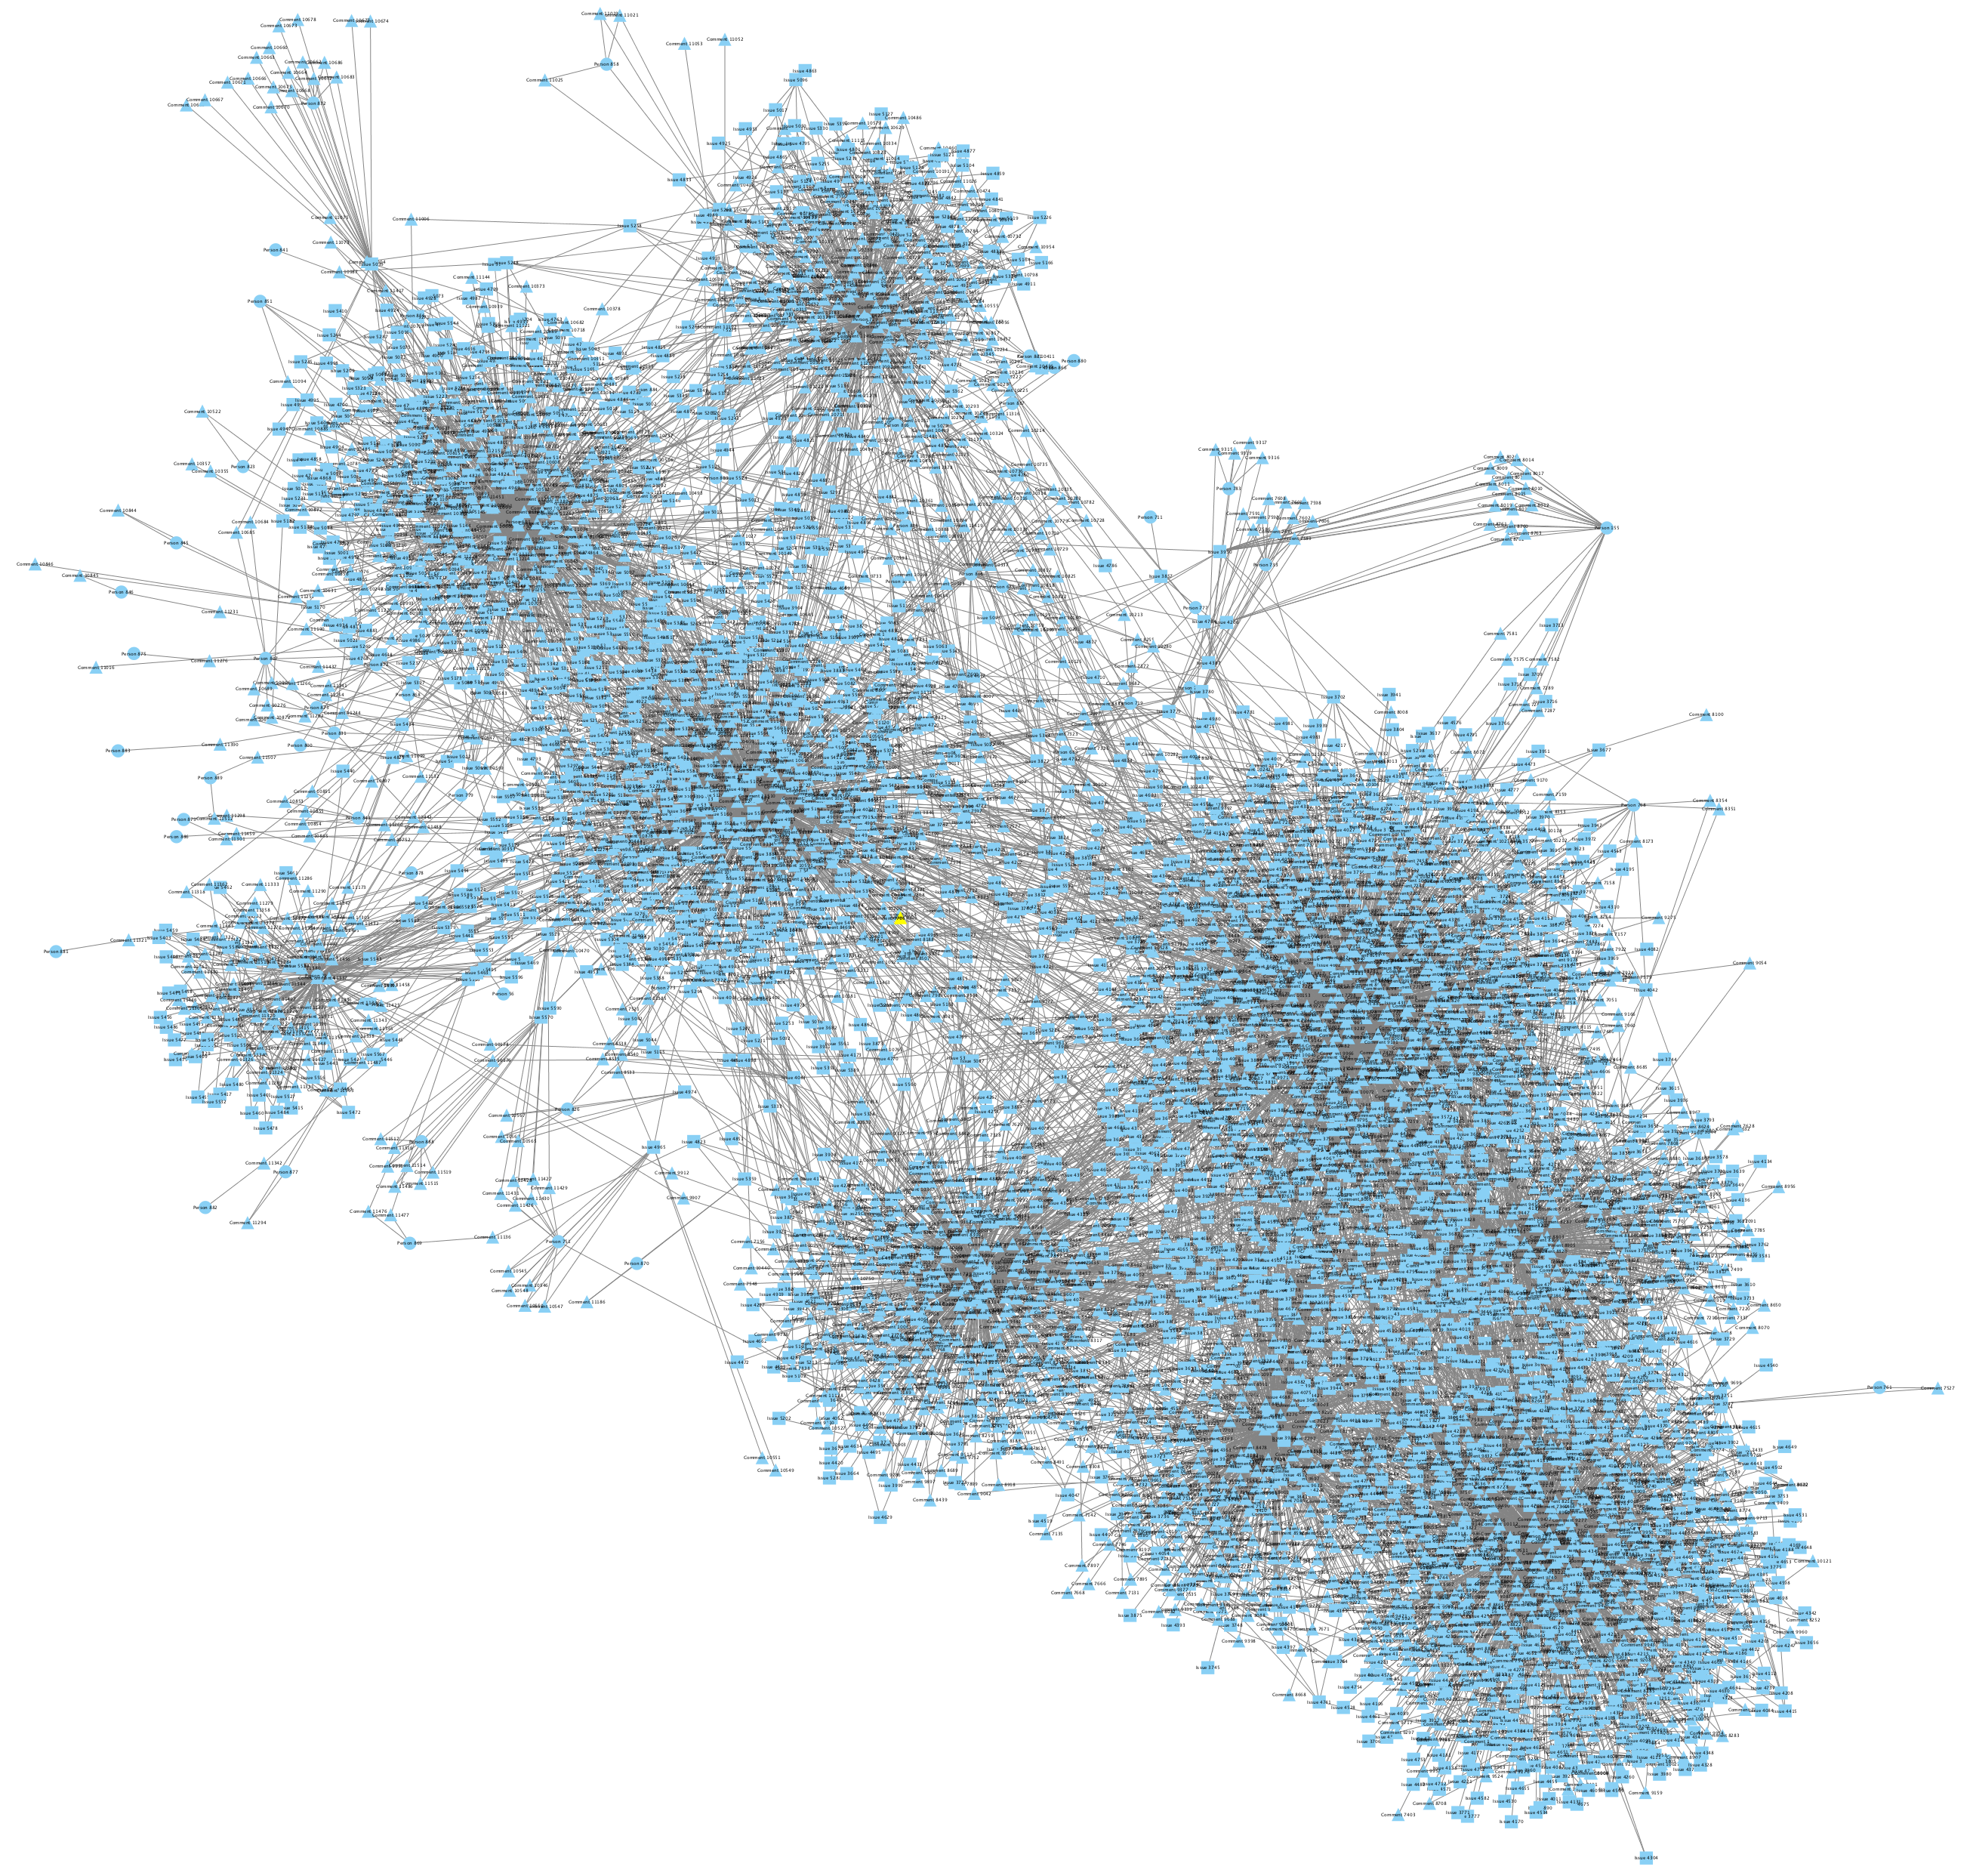
\includegraphics[width=\linewidth]{DegPatch4.pdf}
  \caption{Patch Delineated by 4 Degrees of Socio-Technical Separation}
  \label{fig:degpatch4}
\end{figure}
% \begin{figure}[ht]
%   \centering
%   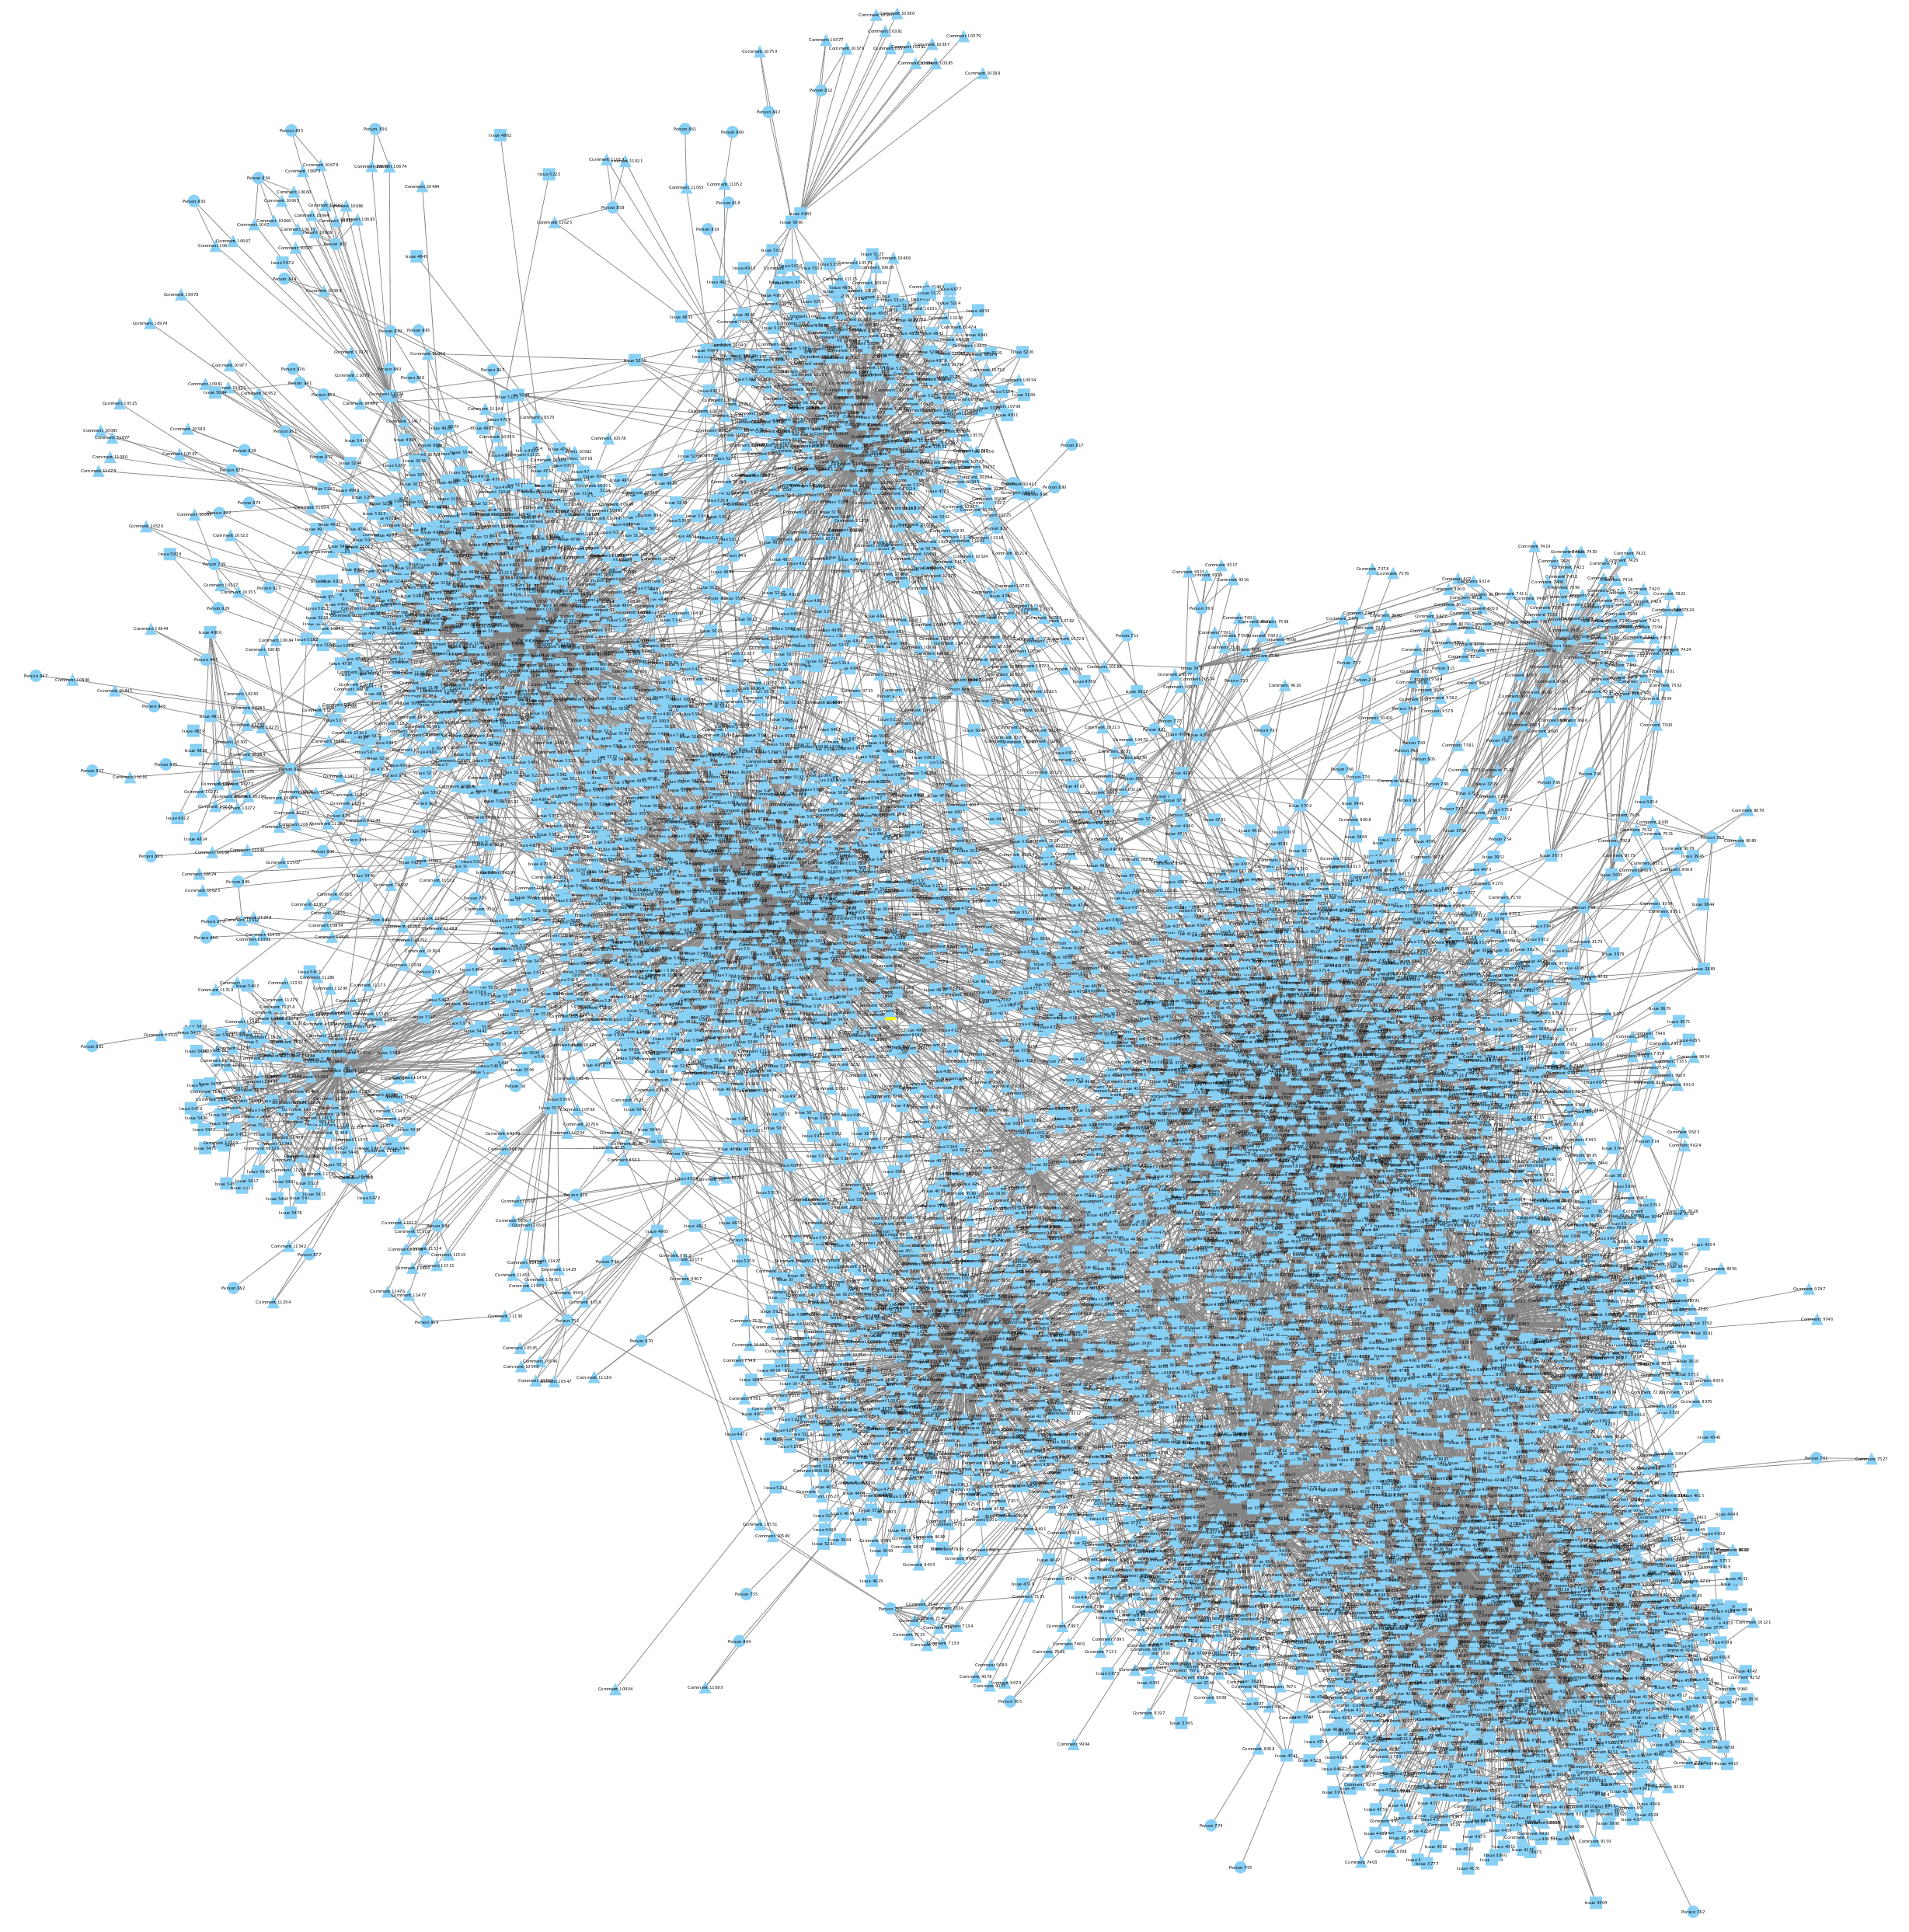
\includegraphics[width=\linewidth]{DegPatch5.pdf}
%   \caption{Patch Delineated by 5 Degrees of Socio-Technical Separation}
%   \label{fig:degpatch5}
% \end{figure}

\begin{figure}[ht]
	\centering
	\includegraphics[width=\linewidth]{c9396weight.png}
	\caption{Example Cytoscape Visualization of Project With Spreading Activation Applied. Darker Nodes Have Higher Activation}
	\label{fig:c9396}
\end{figure}

% \chapter{Jira Examples}
% \label{app:jira}

% \section{Complete DASHBUILDER Answer Set}
% DASHBUILDER was the shortest answer set of our four projects, consisting of 18 Question/Answer pairs. The original answer sets included more columns, including ones that provided evidence of answers. The table below omits these columns, as they weren't used for our script.

% \csvreader[tabular=|l|l|c|l|l|,
%     table head=\hline Body & Asker & Answered & By & Notes \\\hline,
%     late after line=\\\hline]%
% {images/dashbuilder.csv}{Body=\Body,Asker=\Asker,Answered=\Answered,By=\By,Notes=\Notes}%

\chapter{Code}
\label{app:python}

\lstset{ 
  basicstyle=\tiny,                % the size of the fonts that are used for the code
  breaklines=false,                % sets automatic line breaking
  captionpos=b,                    % sets the caption-position to bottom
  keepspaces=true,                 % keeps spaces in text, useful for keeping indentation of code (possibly needs columns=flexible)
  language=Python,                 % the language of the code
  numbers=left,                    % where to put the line-numbers; possible values are (none, left, right)
  numbersep=3pt,                   % how far the line-numbers are from the code
  stepnumber=1,                    % the step between two line-numbers. If it's 1, each line will be numbered
  tabsize=2,                       % sets default tabsize to 2 spaces
  showspaces=false,                % show spaces everywhere adding particular 
}

\begin{singlespace}
\lstinputlisting{../_Scripting/RSTG-SA.py}
\end{singlespace}


\end{document}
